%vim:fo=w
\documentclass[12pt]{../presentation}
\usetheme{default}
\usepackage{ulem}
\usepackage{color}
\usepackage{amsmath}
\usepackage{url}
\usepackage{graphicx}
\usepackage{pgf}
\usepackage{pgfplots}
\pgfplotsset{compat=newest}%
\usepackage{tikz}
\usepackage{apa}
\usetikzlibrary{fit}					% fitting shapes to coordinates
\usetikzlibrary{backgrounds}	% drawing the background after the foreground
\usetikzlibrary{arrows,automata,calc,patterns,snakes}
\usepackage[latin1]{inputenc}
\usepackage{verbatim}
\usepackage{color, colortbl}
\newcommand{\putgraphic}[4]{%
\begin{figure}
\begin{center}
	\includegraphics[width=#4\textwidth]{#1}
\end{center}
	\caption{#2} \label{fig:#3}
\end{figure}}




\newcommand{\vocab}{\mathbf{v}}
\newcommand{\dtvec}{\mathbf{t}_\Delta}
\newcommand{\ctxvec}{\mathbf{t}_\text{ctx}}
\newcommand{\dt}{\Delta_t}
\newcommand{\prerror}{Pr_{error}}
\newcommand{\weights}{\mathbf{w}}
\newcommand{\X}{\mathbf{X}}
\newcommand{\post}{\rho}
\renewcommand{\t}{t}
\newcommand{\w}{w}

\newcommand{\Prerror}{Pr_{\text{error}}}

\newcommand{\Z}{\mathbf{Z}}
\newcommand{\W}{\mathbf{W}}

\newcommand{\pcite}[1]{\textcolor{darkblue}{\cite{#1}}}
\newcommand{\outpcite}[1]{\textcolor{darkblue}{\outcite{#1}}}
\setbeamertemplate{footline}{~\insertframenumber/\inserttotalframenumber}
\title{Predicting Web 2.0 Thread Updates}
\author{Shawn Tan}
%HIghlight clearly contributions.
% Slide numbers. FIX!!
% Show examples to motivate
% 
\AtBeginSection[]
{
	\begin{frame}{Contents}
	\tableofcontents[currentsection]
	\end{frame}
}
\date{22$^\text{nd}$ November 2012}
\setbeamercolor{uppercolgreen}{fg=black,bg=green!35}
\setbeamercolor{lowercolgreen}{fg=black,bg=green!10}
\begin{document}
\maketitle
\section{Introduction}
	\begin{frame}{Motivation}

%Motivate more, important for this data to be crawled close to real-time
	\only<1>{
		Why predict updates?
		\begin{enumerate}
			\item Increase in number of sites with discussion threads
			\item Keeping up to date with information in discussion threads
			\item Incremental crawlers
	\end{enumerate}}
	\only<2>{
		What do we need to do?\\
		Balance:
		\begin{itemize}
			\item Bandwidth consumption
				\begin{itemize}
				\item Cannot repeatedly visit page at short intervals
				\end{itemize}
			\item Timeliness of visits
				\begin{itemize}
					\item Visiting at too large intervals causes data to be not 
						fresh.
				\end{itemize}
		\end{itemize}}
\only<3>{
	Contributions
	\begin{enumerate}
\item Provided evaluation metrics that can be parameterised
\item Proposed methods that perform better than the baseline, and can be employed for making revisit time estimation.
	\end{enumerate}}
	\end{frame}

\section{Related Work}
%ORGANISE!
% Introduce the related work
	\begin{frame}{Revisitation Policies}
		\outpcite{Coffman1997}
		\begin{itemize}
	\item Follows Poisson process $\Rightarrow$ revisit at times proportional to 
		$\mu$ is optimal
		\end{itemize}
	\end{frame}
	\begin{frame}{Empirical evaluations}
		Performed by Cho and Garcia-Molina
		\begin{itemize}
			\item Showed empirically that the Poisson process model estimates 
the update processes well \pcite{Cho1999}
	\item Proposed different revisiting or refresh policies 
\pcite{Cho2003,Garcia-molina2003}
	\end{itemize}
	\end{frame}
	\begin{frame}
		%Use pictures to describe how the sitemap looks, the index of forums 
		%look, and how it helps with the revisits.
	\outpcite{Brian2000} show that page updates are not memoryless, so do not 
	strictly follow  a Poisson process.
	\end{frame}
	\begin{frame}
		\outpcite{Yang2009}
	\begin{enumerate}
		\item Infer a sitemap.
		\item Use a linear-regression model to rank when to next visit
		\item Linear model used together with the sitemap information to 
prioritise the request queue in the crawler.
	\end{enumerate}
Has the ability to make use of index information to infer changes in threads.  
Other types of comment systems do not have such indices.\\
~\\
What about content?
	\end{frame}

	\begin{frame}{Content for prediction}
		%consider using this for intro
\only<1>{
	\begin{center}
		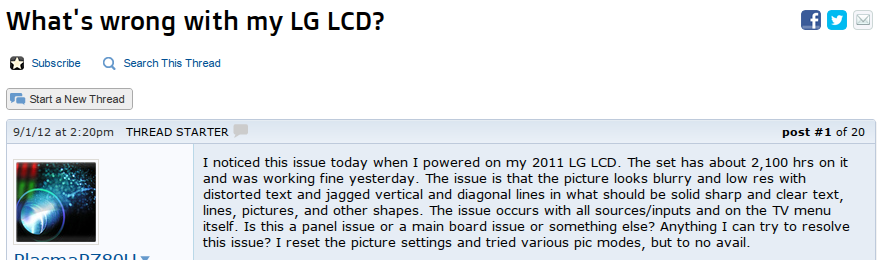
\includegraphics[scale=0.3]{screenshots/question.png}\\
			$\vdots$\\
		
\includegraphics[scale=0.3]{screenshots/question2.png}
	\end{center}}
\only<2>{
	\begin{center}
		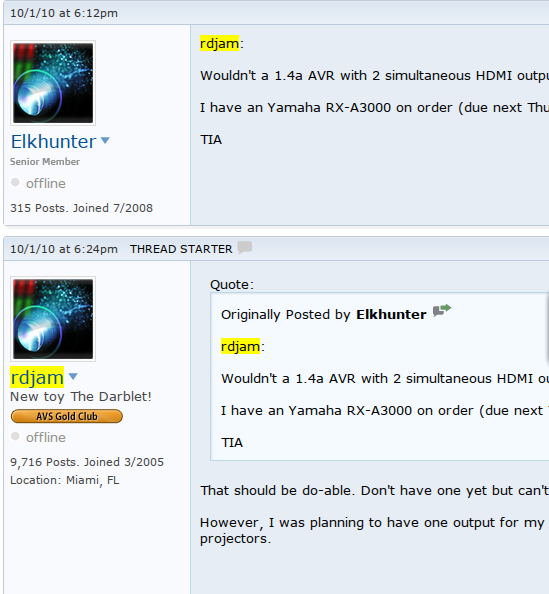
\includegraphics[scale=0.4]{screenshots/replies.png}\\
	\end{center}}
	\end{frame}

	\begin{frame}{Evaluation Metrics}
		% Must go through the contributions again.
		% Do this par twith eval metric section

		% Shorten, don't put too much description
		\begin{enumerate}
			\item \outpcite{Yang2009} $T$-score metric, but dependent on 
				bandwidth
			\item Weighted sum of probability of misses and false alarms used by 
				segmentation metric in \outpcite{Georgescul2009}. Not useful for 
				measuring time differences.
		\end{enumerate}
	\end{frame}
	
	%TODO: shift entire evaluation metrics here.

	\begin{frame}{Summary}
		\begin{itemize}
			\item Visiting at average update rate may not be suitable for 
user-generated content.
			\item Does not make use of content in prediction.
			\item Evaluation metrics not suitable for comparison
		\end{itemize}
	\end{frame}
\section{Evaluation Metric}
	\begin{frame}{Requirements}
		\begin{enumerate}
			\item Balance:
				\begin{itemize}
				\item Bandwidth consumption
				\item Timeliness of visits
				\end{itemize}
			\item Parameterised such that can attribute different importance to 
both
			\item Simple metric to compare across algorithms
		\end{enumerate}
	\end{frame}
	\begin{frame}{Visit/Post ratio}
				\[ \frac{\text{Number of Visits}}{\text{Number of Posts}} \]
		\begin{itemize}
			\item Get an idea of how many number of visits needed before a post 
				is retrieved.
		\end{itemize}
	\end{frame}
	\begin{frame}{$T$-score}
		% put legend
	\begin{center}
		\input{diagrams/t_score_diag}
	\end{center}
	\end{frame}
	\begin{frame}{How do we compare?}
		\begin{itemize}
			\item Two different metrics
				\begin{itemize}
					\item Visit/Post ratio
					\item $T$-score
				\end{itemize}
			\item Problem: how to compare?
				\begin{itemize}
					\item One may be higher than the other
					\item $T$-score / Bandwidth may be less important
					\item Not on the same scale of things, don't represent 
						similar units
				\end{itemize}
		\end{itemize}
	\end{frame}
	\begin{frame}{Worst-case $T$-score ($T_\text{max}$)}
	\begin{center}
		\input{diagrams/norm_t_score_diag}
	\end{center}
	\begin{enumerate}
		\item Assume a visit at the last post.
		\item $T$-score in this case would be the maximum possible
	\end{enumerate}
	\end{frame}
	\begin{frame}{Worst-case Visit/Post ratio}
	\begin{center}
		\input{diagrams/fa_diag}
	\end{center}
	\begin{enumerate}
		\item Assume a discrete time unit (minutes).
		\item For every time unit that a post does not appear in, assume a visit 
			appears.
		\item Visit/Post ratio in this case would be the maximum possible.
		\end{enumerate}
	\end{frame}
	\begin{frame}{$\prerror$}
		%Explain more about what FA and miss means a bit.
		\begin{itemize}
			\item Take ratio:
				\begin{itemize}
					\item $
							{Pr}_{\text{FA}} = 
							\dfrac{\text{P/V-ratio}}{\text{Maximum P/V-ratio}}
						$\\
					\item $
							{Pr}_{\text{miss}} = \dfrac{T}{T_\text{max}}
						$
				\end{itemize}
			\item Weighted sum of both metrics:	\[
				\prerror = \alpha {Pr}_{\text{FA}} + 
(1-\alpha){Pr}_{\text{miss}}
			\]
			\item $0 \leq \alpha \leq 1$
		\end{itemize}
	\end{frame}


\section{Method}
%Explain how the predictions are done: regression, what data i have.. 
\subsection{Features}

\begin{frame}
	\huge Features
\end{frame}
	\begin{frame}{What features?}
		%High level introduction of what type of features are being used...
		% Novelty is use of content.
		% Online algorithm.. 
	\begin{itemize}
		\item Single post: features too sparse, too little information
		\item $w$ recent posts: more indicative of current state of thread.
	\end{itemize}
	\end{frame}
	\begin{frame}{Windowing}
		\begin{center}
		\tikzstyle{background}=[rectangle,
	fill=gray!10,
	inner sep=0.2cm,
	rounded corners=5mm]


\tikzstyle{post}=[circle,
	thick,
	minimum size=0.75cm,
	draw=blue!80,
	fill=blue!20]
% The measurement vector is represented by an orange circle.
\tikzstyle{visit}=[circle,
	thick,
	minimum size=0.75cm,
	draw=orange!80,
	fill=orange!25]

\begin{tikzpicture}[>=latex,text height=1.5ex,text depth=0.25ex]
    % "text height" and "text depth" are required to vertically
    % align the labels with and without indices.
  
  % The various elements are conveniently placed using a matrix:
  \matrix[column sep=0.3cm] {
    % First line: Control input
    	&
		\node (e0)					{};&
		\node (e1)	[post]			{}; &
		\node (e2)	[visit]			{}; &
		&&
		\node (e3)	[post]			{}; &
		\node (e4)	[post]			{}; &
		&&
		\node (e5)	[visit]			{}; &
		\node (e6)	[post]			{}; &
		\node (e7)	[visit]			{}; &
		\node (e)					{};&
		&
        \\
	};
    
    % The diagram elements are now connected through arrows:

	\path[-]
		(e0) edge[thick]	(e1)
		\foreach \e in {1,2,3,4,5,6}{
			let \n1={int(\e+1)} in (e\e) edge[thick] (e\n1)
		}
		(e7) edge[thick]	(e)
	;
	\begin{pgfonlayer}{background}
		\only<1>{\node [background,fit=(e1) (e3)] {};}
		\only<2>{\node [background,fit=(e3) (e4)] {};}
		\only<3>{\node [background,fit=(e4) (e6)] {};}
    \end{pgfonlayer}


\end{tikzpicture}

		\end{center}
		\begin{itemize}
			\item \textcolor{blue}{Posts}
			\item \textcolor{orange}{Visits}
			\item \textcolor{lightgray}{Window}
		\end{itemize}
	\end{frame}
	\begin{frame}{Window time intervals ($\dtvec$)}
		\begin{itemize}
			\item Time intervals between posts inside window
			\item \outpcite{Yang2009}
		\end{itemize}
	\end{frame}
	\begin{frame}{Time context ($\ctxvec$)}
		\begin{itemize}
			\item Day of week and hour of day (bit vector)
				\[
					\underbrace{[0,0,\hdots,1,\hdots0]}_{\text{length of 24}}
				\]
			\item \outpcite{Yang2009}
	\end{itemize}
	\begin{center}
		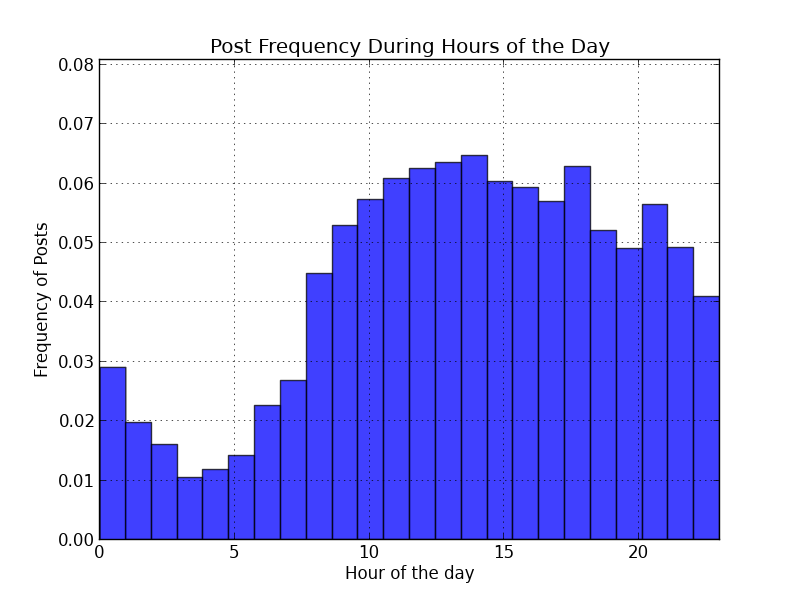
\includegraphics[width=0.4\textwidth]{diagrams/hoursofday.png}
		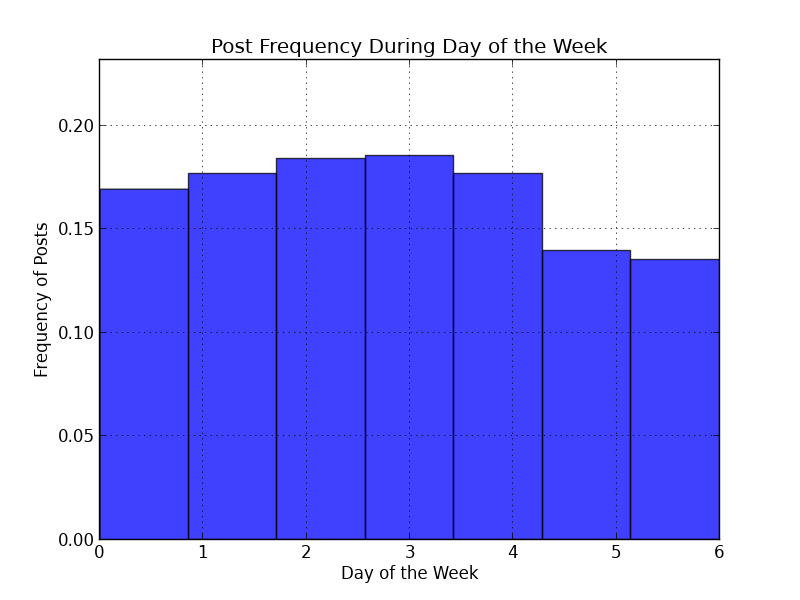
\includegraphics[width=0.4\textwidth]{diagrams/daysofweek.png}
	\end{center}
	\end{frame}
	\begin{frame}{Content Features ($\vocab$)}
	\begin{itemize}
		\item Term occurrence counts.
		\item
		\begin{enumerate}
			\item Text is stemmed, stopwords removed
			\item Occurences of usernames are replaced with `\#USER\#'
			\item Occurences of tokens with mixtures of alphabets and numbers are 
				replaced with `\#MODEL\#'
			\item Univariate regression tests used to select features
		\end{enumerate}
	\end{itemize}
 

	\end{frame}
\begin{frame}
	\huge Algorithms
\end{frame}
\subsection{Algorithms}
	\begin{frame}{Average Revisits (\texttt{BL})}
		\begin{itemize}
			\item Baseline
			\item Average $\dt$ in training set.
		\end{itemize}
	\end{frame}

	\begin{frame}{Support Vector Regression (\texttt{SVR})}
	\begin{itemize}
	\item An extension of using Support Vector Machines for classification
	\item Advantages in high dimension feature vectors \pcite{drucker1997}
	\item Radial Basis Function (RBF) kernel.
	\end{itemize}
	\end{frame}
	\begin{frame}{Stochastic Gradient Descent (\texttt{SGD})}
\only<1>{\begin{itemize}
	\item Linear regression produces poor results -- too big, or negative
	\item Have a function with upper bound ($\Lambda$) and lower bound 
($\lambda$)
	\item Sigmoid function from neural networks
\end{itemize}}
\only<2>{\begin{description}
		\item[Function to be fitted:]
	\[
		f(\X) = \frac{\Lambda-\lambda}{1 + e^{\weights \cdot \X}} + \lambda
	\]
	\item[Update rule:]
	\[
		\Delta \weights_i = \eta
					\underbrace{\left(\widehat{\dt} - \dt \right)}_{\text{error term}}
					\underbrace{\left( f(\X)(1-f(\X)) \right)}_{\text{gradient}}
							\X_i
	\]
	\end{description}}
\only<3>{\begin{center}
	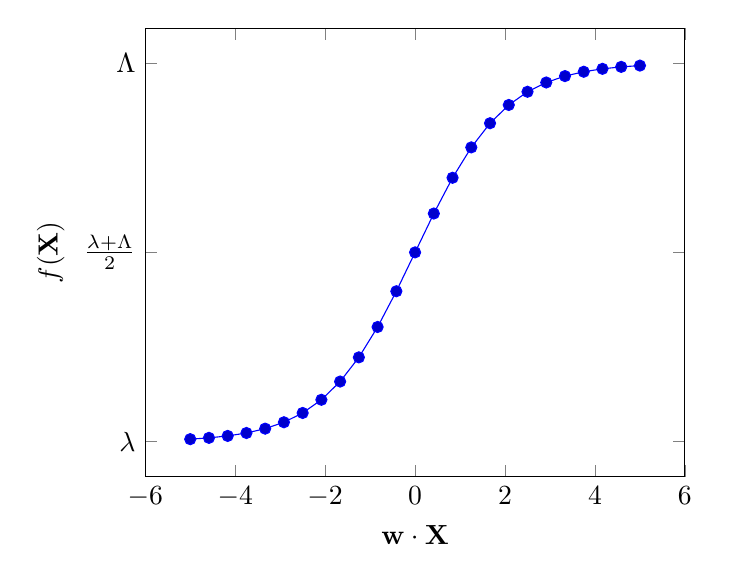
\begin{tikzpicture}
		\begin{axis}[
			xlabel=$\weights\cdot\X$,
			ylabel=$f(\X)$,
			ytick={0,0.5,1},
			yticklabels={$\lambda$,$\frac{\lambda + \Lambda}{2}$,$\Lambda$}
		]
	\addplot {1/(1+ e^-x)}; \end{axis}
	\end{tikzpicture}
	\end{center}}
	\end{frame}
\section{Evaluation}
	\begin{frame}{\url{http://www.avsforum.com/f/}}
		\begin{itemize}
			\item 	4,158 threads 		

			\item 1,002,225 posts 

		\end{itemize}
	\begin{center}
		%log-scale, say truncated
		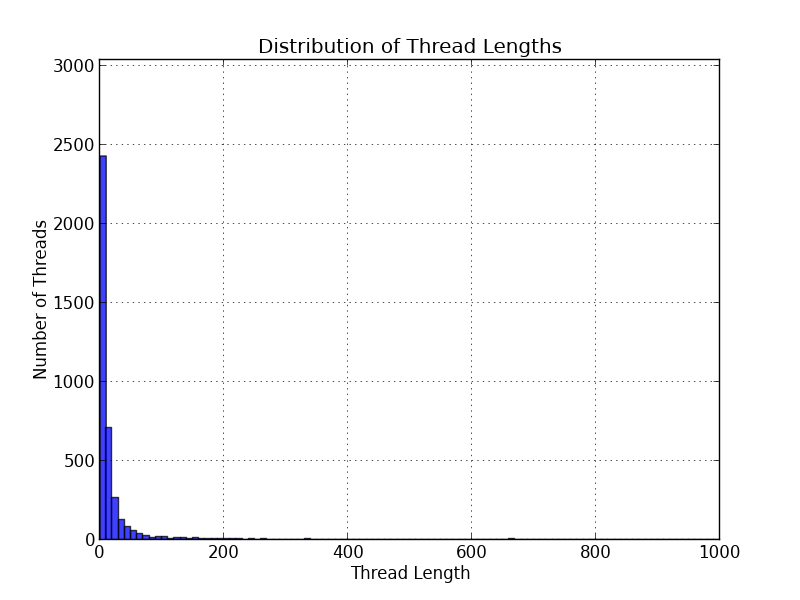
\includegraphics[width=0.6\textwidth]{diagrams/len_dist.png}	
\end{center}
\end{frame}
	\begin{frame}{Experiment setup}
	~\\
	{\scriptsize
	\input{diagrams/exp_setup}
	}
	\end{frame}


	\begin{frame}[t]{Feature set selection}
\begin{beamerboxesrounded}[upper=uppercolgreen,lower=lowercolgreen,shadow=true]{Tuning 
	set}
			\footnotesize
		\begin{enumerate}
			\item Used threads with 100 - 200 posts
			\item Total of 97 threads
			\item Use these to perform tuning
		\end{enumerate}
\end{beamerboxesrounded}
	\only<2>{
		\begin{block}{Using \texttt{SVR}}
		\begin{enumerate}
			\item Window size $w =15$
			\item $\dtvec + \ctxvec + \vocab$ gives best results
				\begin{itemize}
					\item[$\dtvec$] $\dt$ for all time differences in window
					\item[$\ctxvec$] Time context (hour of day, day of week)
					\item[$\vocab$] Word frequencies
				\end{itemize}
		\end{enumerate}
		\end{block}}
	\only<3>{
		\begin{block}{\texttt{SGD} parameter tuning}
			\[
			\Delta \weights_i = \alert{\eta}
						\underbrace{\left(\widehat{\dt} - \dt \right)}_{\text{error term}}
						\underbrace{\left( f(\X)(1-f(\X)) \right)}_{\text{gradient}}
								\X_i
			\]
			\begin{itemize}
				\item Log-scale search
				\item Range: $5\cdot10^{-12} \leq \eta \leq 5\cdot10^{-6} $
				\item Best value: $\eta = 5\cdot10^{-8}$
			\end{itemize}
		\end{block}}
	\end{frame}


	\begin{frame}{Full Evaluation on Dataset}
\begin{center}
\footnotesize
\begin{tabular}{| l | c | c | c | l |}
\hline
& $T$-score			   &	Visit/Post & 	$\prerror$ &\\
\hline
\texttt{SVR}	&	-938.471 $\pm$ 161.545 & 	1.29 $\pm$ 5.207		&	
-0.00728 $\pm$ 0.00327	& $p <  0.05$ \\
\hline
\end{tabular}
\end{center}
	\end{frame}
	\begin{frame}[t]{Full Evaluation on Dataset}
		%Show the baseline performance.
		%Highlight how i make my conclusions.
% Split /	
\begin{beamerboxesrounded}[upper=uppercolgreen,lower=lowercolgreen,shadow=true]{Tuning 
	set}
			\footnotesize
		\begin{enumerate}
			\item Total of 830 threads (Distribution of thread length is long 
				tail)
		\end{enumerate}
\end{beamerboxesrounded}
\only<1>{
\begin{center}
\footnotesize
\begin{tabular}{| l | c | c | c | l |}
\hline
& $T$-score			   &	Visit/Post & 	$\prerror$ &\\
\hline
\texttt{SGD}	&	-479.093 $\pm$ 391.269 & 	1.13 $\pm$ 5.198		&	
-0.00687 $\pm$ 0.00320 	& $p <  0.10$ \\
\hline
\end{tabular}
\end{center}
\begin{enumerate}
	\item \texttt{SVR} method better than baseline.
	\item \texttt{SGD} does not perform as well.
	\item Incurs some `penalty' on the Visit/Post ratio
\end{enumerate}
What if we breakdown the results by thread length?}
% Highlight differences in bar charts...:w
\only<2>{
		\begin{center}
			\tiny
		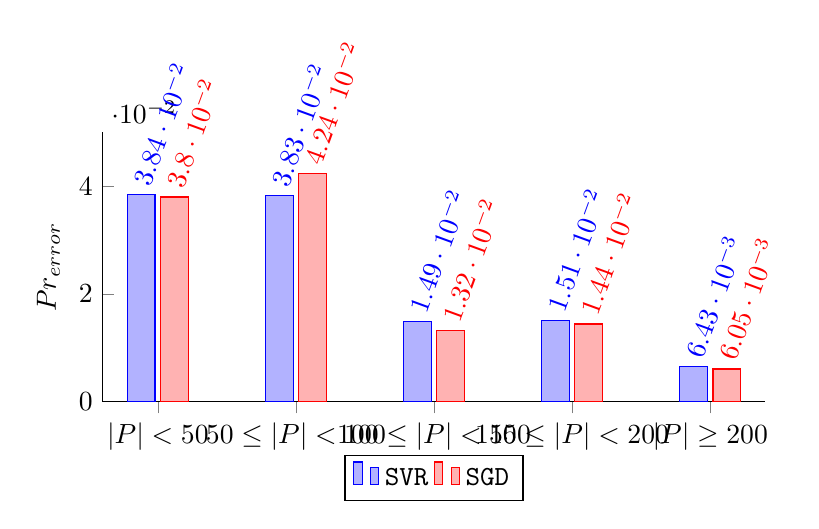
\begin{tikzpicture}
\begin{axis}[
	ybar,
	height=5cm,
	width=10cm,
	enlarge y limits=false,
	axis lines*=left,
	ymin=0,
	ymax=0.05,
	legend style={at={(0.5,-0.2)},
		anchor=north,legend columns=-1},
		ylabel={$\prerror$},
		symbolic x coords={50,100,150,200,201},
		xticklabels={
			$|P| < 50$,
			$50  \leq |P| < 100$,
			$100 \leq |P| < 150$,
			$150 \leq |P| < 200$,
			$|P| \geq 200$
		},
		xtick=data,
		nodes near coords,
		every node near coord/.append style={
			anchor=mid west,
			rotate=70
		}
	]
\addplot coordinates {
	(50,	0.0384)
	(100,	0.0383)
	(150,	0.0149)
	(200,	0.0151)
	(201,	0.00643)
};
\addplot coordinates {
	(50, 	0.0380)
	(100,	0.0424)
	(150,	0.0132)
	(200,	0.0144)
	(201,	0.00605)
};
\legend{\texttt{SVR},\texttt{SGD}}
\end{axis}
\end{tikzpicture}

		\end{center}}
\only<3>{\begin{center}
			\tiny
		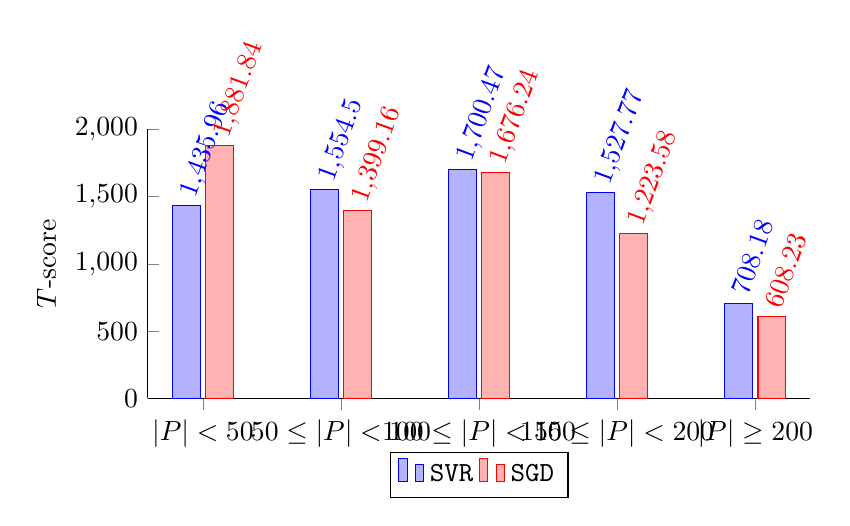
\begin{tikzpicture}
\begin{axis}[
	ybar,
	height=5cm,
	width=10cm,
	enlarge y limits=false,
	axis lines*=left,
	ymin=0,
	ymax=2000,
	legend style={at={(0.5,-0.2)},
		anchor=north,legend columns=-1},
		ylabel={$T$-score},
		symbolic x coords={50,100,150,200,201},
		xticklabels={
			$|P| < 50$,
			$50  \leq |P| < 100$,
			$100 \leq |P| < 150$,
			$150 \leq |P| < 200$,
			$|P| \geq 200$
		},
		xtick=data,
		nodes near coords,
		every node near coord/.append style={
			anchor=mid west,
			rotate=70
		}
	]
\addplot coordinates {
	(50,	1435.96)
	(100,	1554.50)
	(150,	1700.47)
	(200,	1527.77)
	(201,	708.18)
};
\addplot coordinates {
	(50, 	1881.84)
	(100,	1399.16)
	(150,	1676.24)
	(200,	1223.58)
	(201,	608.23)
};
\legend{\texttt{SVR},\texttt{SGD}}
\end{axis}
\end{tikzpicture}

\end{center}}
	\end{frame}
	\begin{frame}{Recommendations \& Limitations}
Recommendations for incremental crawler:
\begin{enumerate}
\item \texttt{SVR} could be used to predict revisitation rates initially, when $|P| < 100$.
\item Later, \texttt{SGD} can be used.
\end{enumerate}
However,
\begin{enumerate}
	\item Experiment results are based on only one dataset
	\item \texttt{SGD} is slow
\end{enumerate}
\end{frame}

\section{Conclusion}
	\begin{frame}{Contributions}
	\begin{enumerate}
	\item Provided evaluation metrics that can be parameterised
	\item Proposed methods that perform better than the baseline, and can be employed for making revisit time estimation.
	\end{enumerate}
	\end{frame}
	\subsection{Future Work}
	\begin{frame}{Topic Modeling}
		\begin{itemize}
			\item Separate window content into different topics
			\item Try to use distribution of $\dt$ in different topics to make prediction
		\end{itemize}
	\end{frame}
	% Show that using words matter..
	\begin{frame}{Natural Language Processing (NLP)}
		Usage of more NLP techniques, like for example in \outpcite{Wang}
		\begin{itemize}
			\item Sentiment analysis
			\item Discourse relation
			\item Sentence similarity
		\end{itemize}
	\end{frame}

\begin{frame}
\begin{center}
	\huge
	Thank you! Questions?
\end{center}
\end{frame}
\bibliographystyle{socreport}
\bibliography{report}

\end{document}

